% Partie hors ligne (Ramy Sail) : corpus, index inversé, distance de Jaccard,
% graphe de seuil, centralités closeness et PageRank, tests.
\section{Partie hors ligne : corpus, index et graphe de Jaccard}
\label{sec:horsligne}

Le précalcul tient en trois étapes du jar, lancées dans cet ordre :
\texttt{corpus} télécharge les livres, \texttt{index} construit l'index inversé,
\texttt{graph} calcule les distances de Jaccard, le graphe et les centralités.
Chaque étape remplace ses tables en une transaction : interrompue, elle laisse
les anciennes intactes. \emph{Méthode de mesure :} deux étapes de mesure
(\texttt{index-scaling}, \texttt{graph-scaling}) exécutent le code de
production sur des échantillons emboîtés de 100 à 2000 livres, tirés au hasard
avec une graine fixe ; après un tour à vide sur le corpus entier, on garde la
médiane de 5 mesures. Machine : Intel Core i7-1360P (16 coeurs) sous WSL, 32Go de
mémoire, Linux, Java~21, PostgreSQL~18 dans Docker.

\subsection{Corpus}
\label{sec:corpus}

\paragraph{Problème et source.} Le sujet demande au moins 1664 livres d'au
moins 10\,000 mots. Ils viennent du projet Gutenberg~\cite{gutenberg}, dont le
catalogue (61\,930 textes anglais sur 79\,712 entrées) donne titre, auteur et
langue. On prend les textes anglais par numéro croissant, surtout des
classiques, plus 49345 et 56667, les deux histoires de la Babylonie de
l'exemple \og Sargon \fg{} du cours. Le site principal interdit
les accès automatisés : les textes viennent du miroir officiel
\texttt{gutenberg.pglaf.org}, un livre toutes les 2~s, soit 4 à 5~heures, avec
reprise après une interruption.

\paragraph{Nettoyage et filtre.} On retire l'en-tête et la licence de
Gutenberg, entre les marqueurs \texttt{*** START OF} et \texttt{*** END OF} :
ces 3\,000 mots, les mêmes partout, mettraient \motif{gutenberg} et
\motif{license} dans toutes les tables et rapprocheraient tous les livres. Un
mot est une suite de lettres Unicode, mots vides compris. Sur 2\,279 livres
examinés, 279 sont écartés : moins de 10\,000 mots, ou absents du miroir.

\paragraph{Résultat.} 2000 livres (numéros 10 à 2430, plus 49345 et 56667), de
10\,016 à 1\,315\,683 mots (médiane 56\,900) : 156~millions de mots, 846~Mo de
texte. Trop gros pour l'archive de 30~Mo, le corpus se reconstruit à
l'identique depuis la liste versionnée \texttt{corpus/ids.txt}. Il garde
quelques éditions en double (deux Bibles du roi Jacques, des pièces de
Shakespeare), qui servent de contrôle : elles doivent être à distance quasi
nulle.

\subsection{Index inversé}
\label{sec:index}

\paragraph{Définitions et structures de données.} La table pondérée d'un livre
$D$ associe à chaque mot $w$ son nombre d'occurrences $k_D(w)$, de somme
$|D|$. Ces tables forment une matrice termes-documents creuse : lue par livre,
c'est l'index direct ; lue par mot, l'index inversé, qui donne la liste des
livres contenant chaque mot. En base de données,
\texttt{term(id, word, book\_count)} numérote le vocabulaire et
\texttt{occurrence(term\_id, book\_id, frequency)}, de clé primaire
$(\mathit{term\_id}, \mathit{book\_id})$, stocke la matrice, une ligne par
couple (mot, livre). Livres et requêtes passent par le même découpage :
normalisation Unicode NFC, coupure sur ce qui n'est pas une lettre (les mots
accentués restent entiers), minuscules, retrait des mots d'une lettre et de 159
mots vides tirés de la liste anglaise de Snowball~\cite{snowball}, qui
domineraient les comptes et rapprocheraient tous les livres.

\paragraph{Algorithme.} Comme dans le cours, l'index direct
d'abord, puis son inversion : (1)~les tables pondérées, en parallèle, une table
de hachage par livre, (2)~le vocabulaire, trié et numéroté par ordre
alphabétique, pour des numéros reproductibles, (3)~l'inversion par tri par
dénombrement : on compte les livres de chaque terme (\texttt{book\_count}), les
sommes cumulées donnent le début de ses lignes, et chaque ligne est rangée à sa
place en parcourant les livres par numéro croissant, soit $O(V \log V + R)$ pour
$V$ termes et $R$ lignes , (4)~le chargement par \texttt{COPY}, clés retirées
puis recréées, pour construire leurs index en une fois et non ligne à ligne.
Chargées dans l'ordre de la clé, les lignes d'un même mot sont contiguës sur le
disque, et la table, relue dans cet ordre, redonne l'index direct de chaque
livre (section~\ref{sec:jaccard}).

\paragraph{État de l'art et choix.} Un index trop gros pour la mémoire se
construit par blocs triés puis fusionnés (BSBI) ou par passes en mémoire
fusionnées sur disque (SPIMI)~\cite{zobel}, \cite[chap.~4]{iir}. Nos
13~millions de lignes tiennent en mémoire : une passe et un tri linéaire
suffisent. Nous gardons tous les mots, même ceux d'un seul livre, puisque le
sujet cherche les livres dont la table contient le mot, mais ni les positions
(pas de recherche de phrases) ni la racine des mots
(section~\ref{sec:conclusion}). La compression des listes relève de la
recherche (section~\ref{sec:motcle}).

\paragraph{Mesures.} La construction en mémoire est linéaire
(figure~\ref{fig:index}) : 0,95~s pour 100 livres, 16~s pour 2000, soit 8~ms par
livre ; le chargement en base ajoute 17~s, pour des tables de 49~Mo
(\texttt{term}) et 834~Mo (\texttt{occurrence}, index compris). Les lignes
croissent aussi linéairement, environ 6\,500 par livre, mais pas le vocabulaire
(figure~\ref{fig:index}, à gauche) : de 100 à 2000 livres, le texte est
multiplié par 20 (de 7,8 à 156~millions de mots), le nombre de termes distincts
par 4 seulement (de 125\,000 à 518\,000), et la courbe s'aplatit. Les 100
premiers livres apportent en moyenne 1\,250 termes nouveaux chacun, les 500
derniers moins de 140, neuf fois moins : les mots courants sont tous vus dès les
premiers livres, et un livre ajouté n'apporte plus que ses mots rares. Ce sont
surtout des noms propres, des mots étrangers et des graphies anciennes ou
dialectales (\emph{abdoolahi}, \emph{praemissus}, \emph{everyzing}) :
281\,000 termes, 54~\% du vocabulaire, n'apparaissent que dans un seul livre,
et 2\,800 seulement dans au moins la moitié des livres.

\begin{figure}[t]
\centering
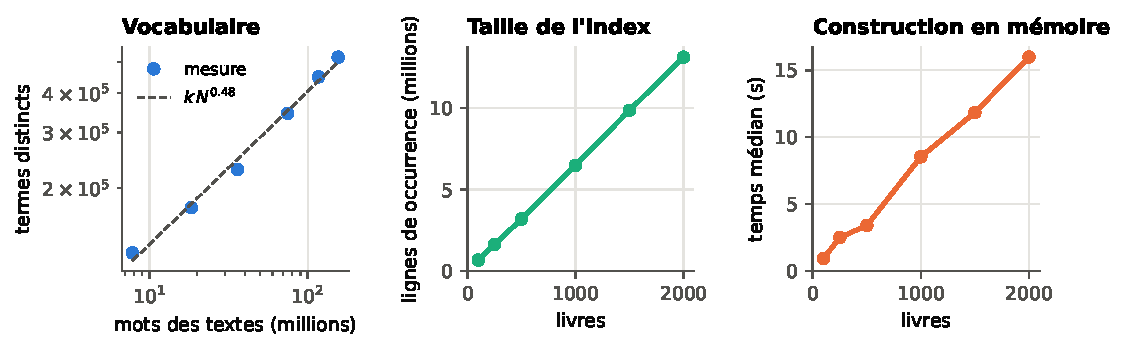
\includegraphics[width=0.9\textwidth]{index-scaling}
\caption{Construction de l'index selon la taille du corpus (échantillons
  emboîtés, médiane de 5 mesures).}
\label{fig:index}
\end{figure}

\subsection{Distance de Jaccard}
\label{sec:jaccard}

\paragraph{Définition.} Le cours compare deux livres par la
distance de Jaccard pondérée, où les sommes portent sur l'union des deux
vocabulaires (un mot absent compte 0 occurrence) :
\[
  d(D_1, D_2)
  = \frac{\sum_w \big(\max(k_1(w), k_2(w)) - \min(k_1(w), k_2(w))\big)}{\sum_w \max(k_1(w), k_2(w))}
  = 1 - \frac{\sum_w \min(k_1(w), k_2(w))}{\sum_w \max(k_1(w), k_2(w))}.
\]
Elle généralise l'indice de Jaccard~\cite{jaccard} $|A \cap B| / |A \cup B|$,
retrouvé quand tous les $k$ valent 0 ou 1. C'est une métrique, nulle pour deux
tables identiques et égale à 1 sans mot commun.

\paragraph{Structure de données et algorithme.} L'étape relit \texttt{occurrence}
dans l'ordre de la clé, par paquets de 50\,000 lignes : les termes de chaque
livre arrivent triés. Chaque livre devient deux tableaux d'entiers triés
(termes, nombres d'occurrences) et son total $|D|$. Une fusion des deux tableaux
donne $\sum \min$ en $O(|V_1| + |V_2|)$, et
$\sum \max = |D_1| + |D_2| - \sum \min$ s'en déduit, puisque
$\max(a, b) = a + b - \min(a, b)$. Les $n(n-1)/2$ paires, 1\,999\,000 pour 2000
livres, sont calculées en parallèle, ligne par ligne de la matrice ($2000^2$
réels, 32~Mo).

\paragraph{État de l'art et choix.} Le calcul exact de toutes les paires est
quadratique. Pour de grands corpus, MinHash~\cite{broder} résume chaque document
par une signature de taille fixe qui estime la similarité de Jaccard, et le
hachage sensible à la localité (LSH) ne compare que des paires
candidates~\cite{mmds} : c'est ainsi qu'on repère les quasi-doublons du Web. Le
cosinus entre vecteurs tf-idf~\cite{iir}, autre mesure courante, est moins
sensible à la longueur des documents. Nous gardons la distance du cours, exacte
et calculée en une demi-minute.

\paragraph{Mesures et exemples.} Le temps croît comme $n^2$
(figure~\ref{fig:graphe-mesures}) : 0,05~s pour 100 livres, 25,6~s pour 2000,
et de 1500 à 2000 livres il est multiplié par 1,80, pour $(4/3)^2 = 1{,}78$
attendu. Extrapolé aux 70\,000 livres de Gutenberg, l'ajustement
$t \approx 6{,}5 \cdot 10^{-6}\,n^2$~s donne 9~heures, les \og heures de calcul
\fg{} du cours : au-delà, il faudrait MinHash. La distance capte le sujet des
livres : les deux histoires de la Babylonie de L.~W.~King (49345, 56667) sont à
0,575, et viennent ensuite, pour 49345, \emph{Legends of Babylon and Egypt}
(0,732) et \emph{History of Phoenicia} (0,736). Les doublons sont presque
confondus : 0,0012 entre les deux Bibles, 0 entre deux \emph{Comedy of Errors}.

\begin{figure}[t]
\centering
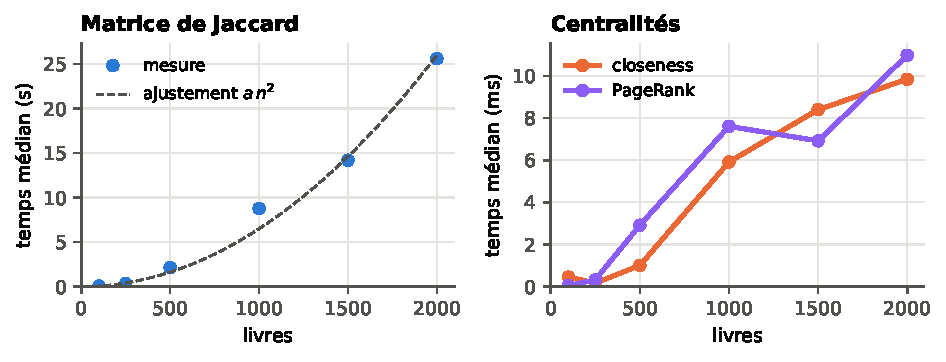
\includegraphics[width=0.72\textwidth]{graph-scaling}
\caption{Temps de calcul du graphe selon le nombre de livres (médiane de 5
  mesures) : la matrice de Jaccard et son ajustement en $n^2$, puis les deux
  centralités.}
\label{fig:graphe-mesures}
\end{figure}

\subsection{Graphe de seuil}
\label{sec:graphe}

\paragraph{Définition et stockage.} Deux livres sont voisins si
$d(u, v) < \theta$, l'arête portant la distance. Les arêtes sont
stockées dans les deux sens dans la table \texttt{neighbor(book\_a, book\_b, distance)},
de clé primaire $(\mathit{book\_a}, \mathit{book\_b})$ : les voisins d'un livre
se lisent par un seul parcours d'intervalle.

\paragraph{Choix du seuil.} Le cours conseille d'ajuster $\theta$ pour un nombre
raisonnable de voisins. Les distances de toutes les paires, triées, donnent par
dichotomie le nombre d'arêtes et de livres isolés pour tout $\theta$
(figure~\ref{fig:seuil}). Nous prenons le plus petit $\theta$ au centième qui
donne un degré moyen d'au moins 20, assez pour les suggestions sans noyer le
graphe : $\theta = 0{,}66$, soit 25\,026 arêtes, un degré moyen de 25 et un
degré maximal de 316. Les distances se concentrent entre 0,7 et 0,95 : seule la
queue gauche de la distribution donne des arêtes.

\begin{figure}[t]
\centering
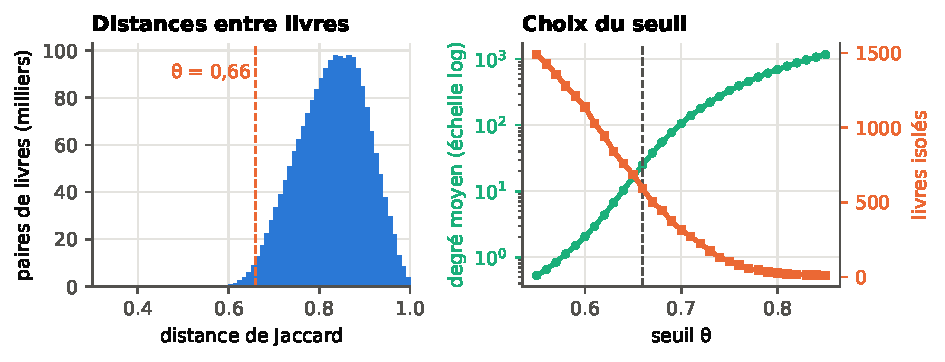
\includegraphics[width=0.72\textwidth]{threshold}
\caption{À gauche, histogramme des distances des 1\,999\,000 paires de livres.
  À droite, degré moyen et nombre de livres isolés selon le seuil ; la ligne
  pointillée marque $\theta = 0{,}66$.}
\label{fig:seuil}
\end{figure}

\paragraph{Structure.} Les 667 composantes connexes retrouvent des genres
(figure~\ref{fig:structure}) : une composante géante de 1027 livres (romans et
recueils de nouvelles), une de 129 (les pièces de Shakespeare, en plusieurs
éditions), une de 35 (la poésie), puis de petites composantes, dont 51 paires,
et 591 livres isolés, soit 30~\% du corpus.

\begin{figure}[t]
\centering
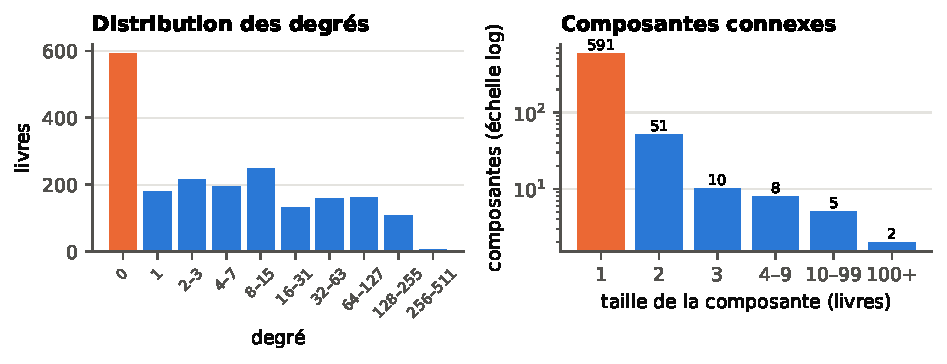
\includegraphics[width=0.72\textwidth]{graph-structure}
\caption{Distribution des degrés (en orange, les livres isolés) et taille des
  composantes connexes, pour $\theta = 0{,}66$.}
\label{fig:structure}
\end{figure}

\paragraph{Les livres isolés.} Ce sont d'abord des livres courts : 169 des 200
plus courts (moins de 18\,500 mots) sont isolés, contre 20 des 200 plus longs,
car un texte court donne une distribution de mots bruitée. Ce sont aussi des
essais, dont les plus proches voisins sont entre 0,70 et 0,76. Normaliser les
comptes par la taille ($k/|D|$), comme le propose le cours, n'améliore pas tant que ça
(521 isolés au lieu de 591, sur un essai ponctuel) ; monter le seuil améliore,
au prix du sens des arêtes (314 isolés à $\theta = 0{,}70$ avec 105 voisins en
moyenne, 26 à 0,80 avec 698). Un corpus plus grand aide : à seuil fixé, la part
des isolés passe de 60~\% sur 100 livres à 30~\% sur 2000. Conséquence dans
l'application : un livre isolé n'a pas de voisin, et les deux livres de
\motif{sargon}, voisins l'un de l'autre seulement, ne donnent aucune
suggestion. Un graphe des $k$ plus proches voisins, qui relie chaque livre à
ses $k$ plus proches quelle que soit leur distance, s'adapte aux régions de
densités différentes : c'est la principale perspective.

\subsection{Centralités : closeness et PageRank}
\label{sec:centralites}

Le sujet impose au moins une centralité parmi closeness, betweenness et
PageRank ; nous en calculons deux, stockées dans la table \texttt{book} pour le
classement (section~\ref{sec:classement}).

\paragraph{Closeness.} Un livre est central s'il est proche de tous les autres :
$C(v) = (n-1) / \sum_{u \neq v} d_G(v, u)$, où $d_G$ compte les arêtes d'un plus
court chemin (ce n'est pas la distance de Jaccard). Notre graphe n'est pas
connexe et $d_G$ y est parfois infinie : nous appliquons la correction de
Wasserman et Faust~\cite{wasserman},
\[
  C(v) = \frac{r - 1}{n - 1} \cdot \frac{r - 1}{\sum_u d_G(v, u)},
\]
où la somme porte sur les $r - 1$ livres atteignables depuis $v$, et
$C(v) = 0$ pour un livre isolé. Sur un graphe connexe ($r = n$), c'est la
formule du cours ; le facteur $(r - 1)/(n - 1)$ pénalise les petites
composantes. La centralité harmonique, $\sum_u 1/d_G(v, u)$, citée par le cours,
accepte aussi les distances infinies, mais ne redonne pas la formule du cours.
\emph{Algorithme :} un parcours en largeur par livre donne $\sum d_G$ et $r$ ;
les $n$ parcours, indépendants, tournent en parallèle, en $O(n(n + m))$.

\paragraph{PageRank.} PageRank~\cite{brin} est la loi stationnaire d'une marche
aléatoire qui, depuis $u$, suit avec la probabilité $\alpha$ une arête vers un
voisin $v$, choisi proportionnellement à la similarité $s(u, v) = 1 - d(u, v)$,
et sinon saute vers un livre quelconque ; la masse des livres isolés, sans arête
à suivre, est redistribuée uniformément. Avec
$S(u) = \sum_w s(u, w)$ et $I$ la masse totale des livres isolés :
\[
  \mathrm{PR}(v) = \frac{1 - \alpha + \alpha I}{n}
  + \alpha \sum_{u \in N(v)} \mathrm{PR}(u)\, \frac{s(u, v)}{S(u)}.
\]
Sans poids, sur un graphe non orienté, la loi stationnaire de la marche est
$\deg(v)/2m$, dont PageRank s'approche quand $\alpha$ tend vers 1 : il redirait
presque le degré ; les poids y ajoutent la proximité des voisins.
\emph{Algorithme :} itération de la puissance depuis la loi uniforme, avec
$\alpha = 0{,}85$, jusqu'à une variation inférieure à $10^{-12}$ en norme $L_1$
(200 itérations au plus). Une itération coûte $O(n + m)$ et l'écart au point
fixe diminue au moins d'un facteur $\alpha$ : 134 itérations sur le corpus.

\paragraph{Pourquoi pas betweenness.} L'algorithme de Brandes~\cite{brandes} la
calcule en $O(nm)$, faisable ici. Mais être sur les plus courts chemins entre
les autres désigne les ponts entre groupes thématiques, pas les livres
représentatifs : pour classer des résultats, closeness et PageRank ont un sens
plus direct.

\paragraph{Mesures.} Closeness prend 9,8~ms et PageRank 11~ms sur 2000 livres
(figure~\ref{fig:graphe-mesures}), contre 25,6~s pour Jaccard : le graphe est
creux ($m \approx 12{,}5\,n$).

\paragraph{Exemple de calcul.} Quatre recueils de poésie australienne, trois de
Banjo Paterson et un d'Henry Lawson (214), forment une composante à part
(figure~\ref{fig:exemple}). Pour 213, $r = 4$ et $\sum d_G = 3$, d'où
$C = \frac{3}{1999} \cdot \frac{3}{3} \approx 1{,}50 \cdot 10^{-3}$ ; pour 214,
$\sum d_G = 1 + 2 + 2 = 5$, d'où $0{,}90 \cdot 10^{-3}$. Sans la correction, 213
vaudrait 1, le maximum possible, loin devant le livre le plus central de la
composante géante, \emph{Novel Notes} (0,240). Pour PageRank, une composante de
$k$ livres est fermée : sa masse $M$ vérifie $M = kJ + \alpha M$, où
$J = (1 - \alpha + \alpha I)/n$ est le saut, commun à tous. D'où
$M = kJ/(1 - \alpha)$ pour toute composante. Comme $I = 591\,J$,
$J = (1 - \alpha)/(n - 591\,\alpha) = 1{,}00 \cdot 10^{-4}$ : un livre relié
vaut en moyenne $6{,}68 \cdot 10^{-4}$, ici comme dans la composante géante, et
un livre isolé seulement $J$. Ici, 213, relié aux trois autres, reçoit 37~\% de
la masse. PageRank pénalise donc les livres isolés, mais pas les petites
composantes, que la closeness corrigée pénalise aussi.

\begin{figure}[t]
\centering
\begin{minipage}[c]{0.42\textwidth}
\centering
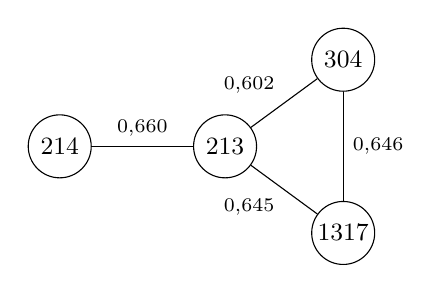
\begin{tikzpicture}[
  book/.style={circle, draw, minimum size=8mm, inner sep=1pt, font=\small},
  dist/.style={font=\scriptsize, midway}]
  \node[book] (a) at (0, 0) {213};
  \node[book] (b) at (-2.1, 0) {214};
  \node[book] (c) at (1.5, 1.1) {304};
  \node[book] (d) at (1.5, -1.1) {1317};
  \draw (a) -- (b) node[dist, above] {0,660};
  \draw (a) -- (c) node[dist, above left] {0,602};
  \draw (a) -- (d) node[dist, below left] {0,645};
  \draw (c) -- (d) node[dist, right] {0,646};
\end{tikzpicture}
\end{minipage}\hfill
\begin{minipage}[c]{0.56\textwidth}
\centering
\small
\begin{tabular}{@{}ccccc@{}}
  \toprule
  Livre & Degré & $\sum d_G$ & Closeness & PageRank \\
  \midrule
  213 & 3 & 3 & $1{,}50 \cdot 10^{-3}$ & $9{,}87 \cdot 10^{-4}$ \\
  304 & 2 & 4 & $1{,}13 \cdot 10^{-3}$ & $6{,}79 \cdot 10^{-4}$ \\
  1317 & 2 & 4 & $1{,}13 \cdot 10^{-3}$ & $6{,}44 \cdot 10^{-4}$ \\
  214 & 1 & 5 & $0{,}90 \cdot 10^{-3}$ & $3{,}61 \cdot 10^{-4}$ \\
  \bottomrule
\end{tabular}
\end{minipage}
\caption{Une composante de quatre livres, avec la distance de Jaccard de chaque
  arête et les centralités dans le graphe complet ($n = 2000$) : \emph{The Man
  from Snowy River} (213), \emph{Rio Grande's Last Race} (304), \emph{Saltbush
  Bill, J.\,P.} (1317), de Paterson, et \emph{In the Days When the World Was
  Wide} (214), de Lawson.}
\label{fig:exemple}
\end{figure}

\paragraph{Comparaison des classements.} Les trois critères placent en tête les
mêmes livres (tableau~\ref{tab:top}) : des recueils de nouvelles d'environ
100\,000 mots, au vocabulaire proche de celui de nombreux romans, et trois
livres de Jerome K. Jerome. PageRank fait monter \emph{Sketches in Lavender,
Blue and Green} au deuxième rang avec 221 voisins seulement : ses voisins ont
eux-mêmes peu de voisins (78 en moyenne, contre 110 pour la \emph{Lock and Key
Library}), et chacun lui transmet une plus grande part de son score. Sur tout
le corpus, les rangs sont très corrélés (Spearman : 0,95 entre degré et
closeness, 0,84 entre degré et PageRank, 0,73 entre closeness et PageRank),
surtout parce que les 591 livres isolés sont derniers partout. Sur les seuls
livres reliés, closeness et PageRank ne s'accordent presque plus (0,26) : la
première favorise le centre de la composante géante, le second les livres qui
reçoivent une grande part du score de leurs voisins, et il donne aux petites
composantes la même moyenne qu'à la grande.

\begin{table}[t]
\centering
\footnotesize
\setlength{\tabcolsep}{5pt}
\begin{tabular}{@{}clrlrlr@{}}
  \toprule
  & \multicolumn{2}{c}{Degré} & \multicolumn{2}{c}{Closeness}
  & \multicolumn{2}{c}{PageRank} \\
  \cmidrule(lr){2-3} \cmidrule(lr){4-5} \cmidrule(l){6-7}
  Rang & Livre & Valeur & Livre & Valeur & Livre & $\times 10^{-3}$ \\
  \midrule
  1 & \emph{Lock and Key Library} I & 316 & \emph{Novel Notes} & 0,240 & \emph{Novel Notes} & 3,76 \\
  2 & \emph{Novel Notes} & 296 & \emph{Lock and Key Library} I & 0,238 & \emph{Sketches in Lavender\dots} & 3,23 \\
  3 & \emph{All Roads Lead to Calvary} & 271 & \emph{Beauty and the Beast\dots} & 0,236 & \emph{Lock and Key Library} I & 3,17 \\
  4 & \emph{Lock and Key Library} II & 265 & \emph{Lock and Key Library} II & 0,235 & \emph{Beauty and the Beast\dots} & 2,74 \\
  5 & \emph{St. Ives} & 260 & \emph{St. Ives} & 0,235 & \emph{Lock and Key Library} II & 2,74 \\
  \bottomrule
\end{tabular}
\caption{Les cinq livres les plus centraux selon chaque critère, sur le corpus
  complet. \emph{Lock and Key Library} : I, \emph{Modern English} ; II,
  \emph{Old Time English}.}
\label{tab:top}
\end{table}

\subsection{Tests}
\label{sec:testshorsligne}

73 tests JUnit couvrent la partie hors ligne, sur des jeux d'essai du
cours ou construits pour le test, aux valeurs calculées à la
main :
\begin{itemize}[nosep]
  \item découpage en mots et nettoyage d'un petit texte construit avec les
        marqueurs de Gutenberg ;
  \item index : D1 à D3 du cours redonnent exactement les tables du jeu
        d'essai, dans n'importe quel ordre ;
  \item Jaccard : les distances du cours (0,75, 15/16, 10/13), 0 entre tables
        identiques, 1 sans mot commun ; graphe : aucune arête à $\theta = 0{,}5$,
        le chemin D1 -- D3 -- D2 à 0,8, le triangle à 1 ;
  \item closeness : les huit valeurs du graphe A à H du cours ($7/11$ pour E,
        $7/18$ pour G\dots), deux composantes et un sommet isolé ;
  \item PageRank : somme égale à 1, $1/n$ sur un cycle, $0{,}88/1{,}85$ au
        centre d'une étoile à quatre feuilles, poids égaux identiques à
        l'absence de poids ;
  \item étapes complètes sur un PostgreSQL jetable (Testcontainers) : index et
        graphe du jeu d'essai reconstruits à l'identique, centralités comprises.
\end{itemize}
Sur le corpus complet, la somme des PageRank vaut 1 à $10^{-12}$ près, et les
doublons connus sont à distance quasi nulle.
